../cictikz/src/cictikz/data/tex/cictikz_preamble.tex

% The open source IC design flow, landscape: analog path in red, digital
% path in blue, from Idea to Tapeout.

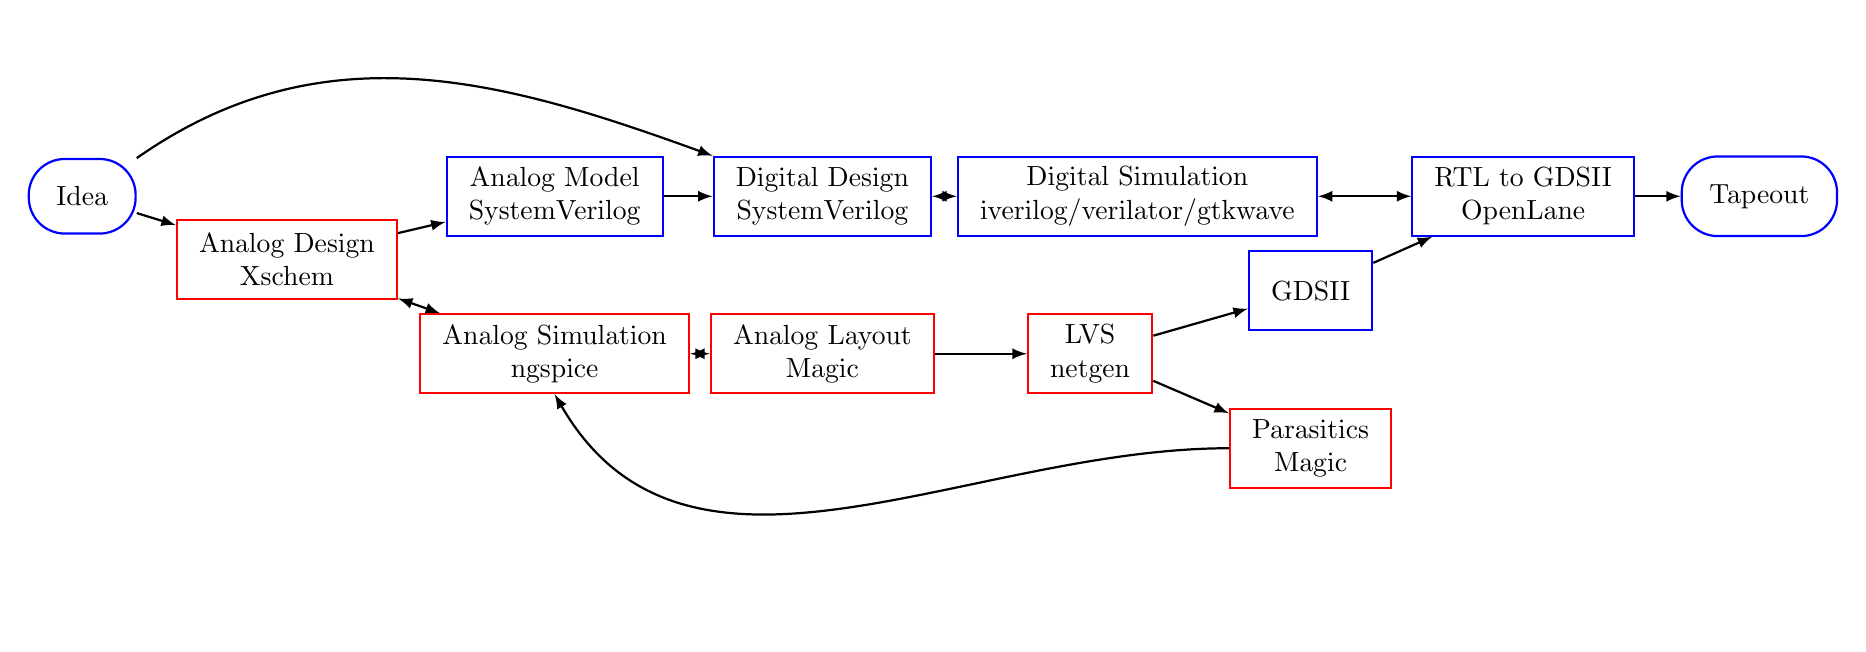
\begin{tikzpicture}[thick,
  ana/.style={draw=red, rectangle, align=center, minimum height=1.0cm,
              inner xsep=8pt},
  dig/.style={draw=blue, rectangle, align=center, minimum height=1.0cm,
              inner xsep=8pt},
  term/.style={draw=blue, rectangle, rounded corners=13pt, align=center, inner sep=10pt},
  a/.style={-latex},
  ab/.style={latex-latex}]

  \node[term] (idea)   at (-0.4,2.6)  {Idea};
  \node[ana]  (xschem) at (2.2,1.8)   {Analog Design\\Xschem};
  \node[dig]  (amod)   at (5.6,2.6)   {Analog Model\\SystemVerilog};
  \node[ana]  (asim)   at (5.6,0.6)   {Analog Simulation\\ngspice};
  \node[dig]  (ddes)   at (9.0,2.6)   {Digital Design\\SystemVerilog};
  \node[ana]  (alay)   at (9.0,0.6)   {Analog Layout\\Magic};
  \node[dig]  (dsim)   at (13.0,2.6)  {Digital Simulation\\iverilog/verilator/gtkwave};
  \node[ana]  (lvs)    at (12.4,0.6)  {LVS\\netgen};
  \node[dig]  (gds)    at (15.2,1.4)  {GDSII};
  \node[ana]  (par)    at (15.2,-0.6) {Parasitics\\Magic};
  \node[dig]  (lane)   at (17.9,2.6)  {RTL to GDSII\\OpenLane};
  \node[term] (tape)   at (20.9,2.6)  {Tapeout};

  \draw[a]  (idea) -- (xschem);
  \draw[a]  (idea) to[out=35, in=160] (ddes.north west);
  \draw[a]  (xschem) -- (amod);
  \draw[ab] (xschem) -- (asim);
  \draw[a]  (amod) -- (ddes);
  \draw[ab] (ddes) -- (dsim);
  \draw[ab] (asim) -- (alay);
  \draw[a]  (alay) -- (lvs);
  \draw[a]  (lvs) -- (gds);
  \draw[a]  (lvs) -- (par);
  \draw[a]  (par) to[out=180, in=-60] (asim.south);
  \draw[a]  (gds) -- (lane);
  \draw[ab] (dsim) -- (lane);
  \draw[a]  (lane) -- (tape);

\end{tikzpicture}
\end{document}
